% \begin{saveblock}{providesclass}
% 	\begin{highlightblock}[gobble=8,linewidth=\textwidth,
% 		framexleftmargin=0.25em,xleftmargin=0.25em]
%         % Bestand: inleveropgave.cls
% 		\NeedsTeXFormat{LaTeX2e}
%         \ProvidesClass{inleveropgave}
%         [2021/10/26 inleveropgave v1.0]

%         \LoadClass[a4paper]{article}
%         \RequirePackage{amsmath,amssymb,amsthm}
%         \RequirePackage[margin=2.54cm]{geometry}
%         ...
% 	\end{highlightblock}
% \end{saveblock}

% \begin{saveblock}{documentclass}
%     \begin{highlightblock}[gobble=8,linewidth=\textwidth,
% 		framexleftmargin=0.25em,xleftmargin=0.25em]
%         % Bestand: document.tex
%         \documentclass{inleveropgave}
%         \begin{document}
%             Hey!
%         \end{document}
%     \end{highlightblock}
% \end{saveblock}

% \begin{frame}{Class}
%     \useblock{providesclass}

%     \medskip

%     \useblock{documentclass}
% \end{frame}

\copyrightVincent
\begin{frame}[fragile]{Aparte preamble, optie 2: eigen documentclass}
    \begin{columns}
        \begin{column}{0.5\textwidth}
            \small
            Bestand \texttt{document.tex}:
            \begin{minted}[fontsize=\scriptsize]{tex}
                \documentclass{inleveropgave}
        
                \begin{document}
                    ...
                \end{document}
            \end{minted}
        \end{column}
        \begin{column}{0.5\textwidth}
            \small
            Bestand \texttt{inleveropgave.cls}:
            \begin{minted}[fontsize=\scriptsize]{tex}
                \NeedsTeXFormat{LaTeX2e}
                \ProvidesClass{inleveropgave}
                [2022/10/17 inleveropgave v1.0]

                \LoadClass{article}
                \RequirePackage[a4paper,margin=2.54cm]{geometry}
                \RequirePackage{amsmath}
                \RequirePackage{amssymb}
                ...
            \end{minted}
        \end{column}
    \end{columns}
\end{frame}

\begin{frame}[fragile]{Aparte preamble, optie 2: eigen documentclass}
    \begin{center}
        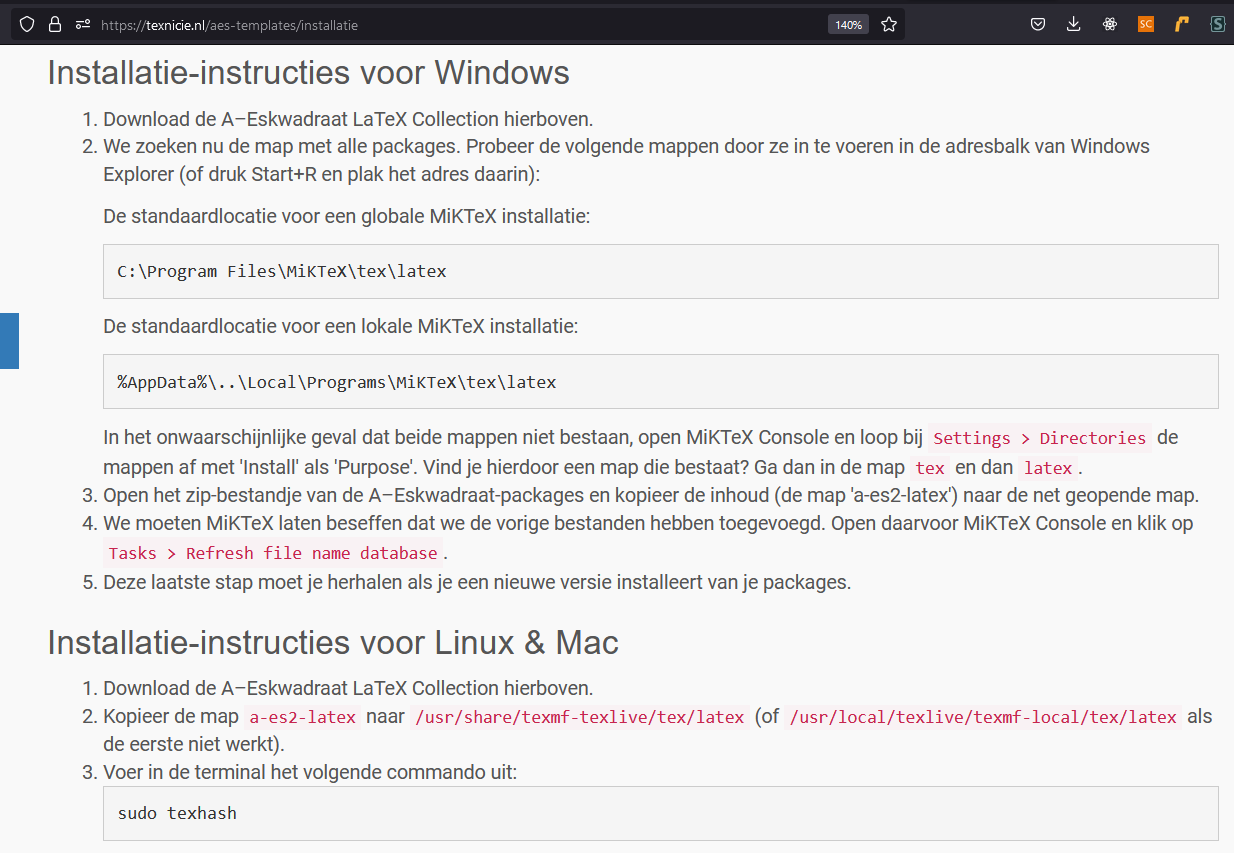
\includegraphics[height=0.8\textheight]{assets/aesTemplatesManualInstallation_wide.png}
    \end{center}
\end{frame}
